\section{Experimentación Computacional}

Los resultados fueron producidos usando conjuntos de datos sintéticos y reales en una máqina
Dell OPTIPLEX 7010 con procesador Intel\textregistered Core\texttrademark  i7-3770 CPU de 3.40GHz x 8,
16 GB de RAM y 1TB 7200 RPM de Disco Duro, corriendo Ubuntu con linux 3.5. Para todos los casos se usaron
los algoritmos implementados en python version 3.

\subsection{San Joaquin}

Un grupo de conjuntos de datos sintéticos fueron creados usando un modelo para la generación de objetos en movimiento, como se describe en \cite{brinkhoff2002framework}.
Dos conjuntos de datos sintéticos fueron creados usando la red de San Joaquín proporcionada en el sitio web del generador basado en red \cite{Brin:2010:Online}.
El primer conjunto de datos recoge 992140 lugares simulados para 25.000 objetos en movimiento durante 60 instantes de tiempo. El segundo recoge 50.000 trayectorias
de 2.014.346 de puntos durante 55 instantes de tiempo. La Table~\ref{tab:datasets} resume la información principal. Es importante aclarar que el tamaño de la trayectoria se refiere al
número promedio de ubicaciones de puntos e intervalos de tiempo en lugar de a la longitud espacial media.


\begin{table}
\caption{Conjunto de datos sintéticos}
\label{tab:datasets}
\centering
\scalebox{0.8}{
\begin{tabular}{c c r r c}
\toprule
\multirow{2}{*}{Dataset}& \multirow{2}{*}{Network}& \multicolumn{1}{c}{Number of}& Number of  & Trajectory\\
                        &                         & Trajectories & \multicolumn{1}{c}{Points} & size (avg)\\
\midrule
SJ25KT60  & San Joaquin & 25000 & 992140  & 40\\
SJ50KT55  & San Joaquin & 50000 & 2014346 & 37\\
TAPAS Cologne  & Cologne, Germany & 49225 & 1813454 & 37\\
Original\_Beijing   & Beijing, China   & 23800 & 1207110 & 50\\
Alternative\_Beijing   & Beijing, China   & 18216 & 760814 & 42\\
\bottomrule
\end{tabular}}
\end{table}

\begin{figure}
  \centering
  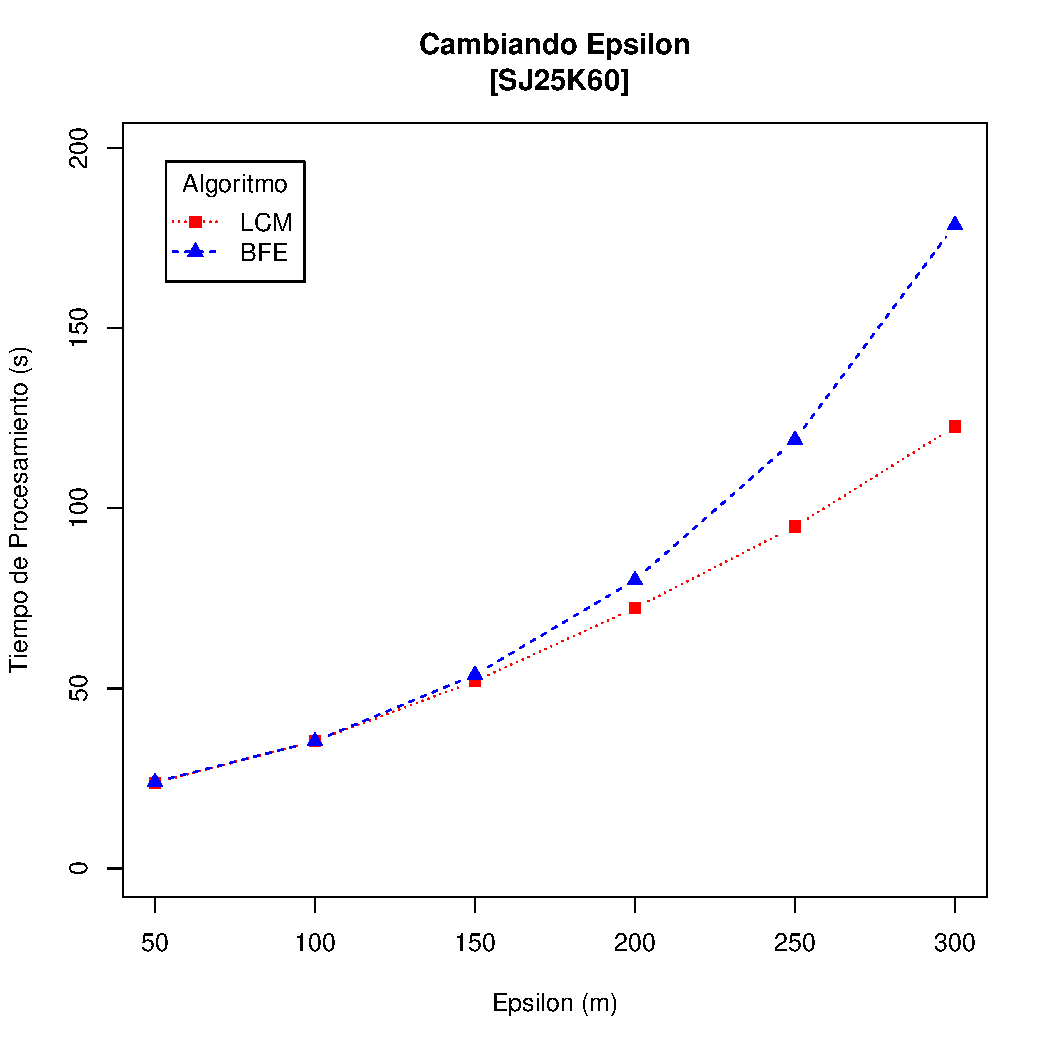
\includegraphics[scale=0.4]{pictures/SJ25K60.pdf}
  \caption{Caso de Prueba: SJ25K60}
  \label{fig:SJ25K60}
\end{figure}

\begin{figure}
  \centering
  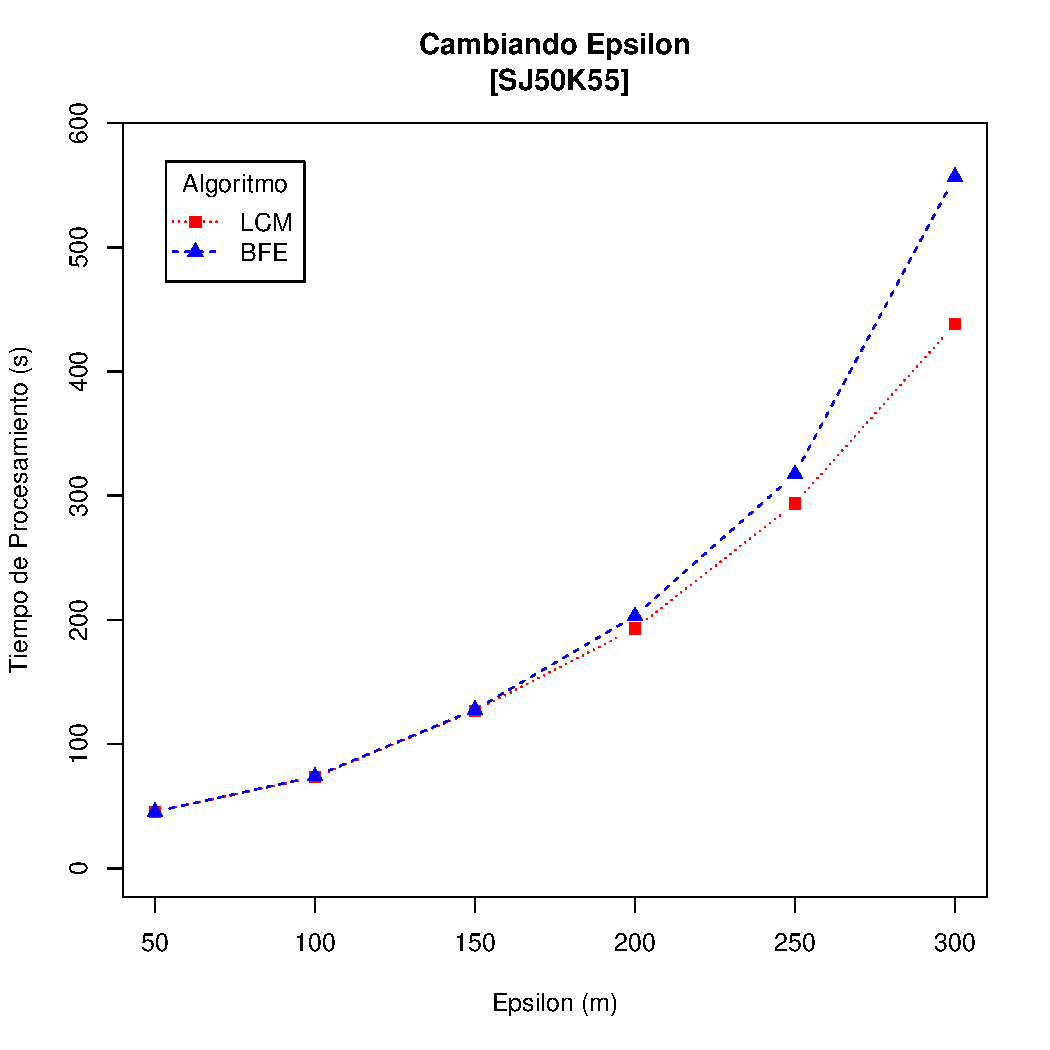
\includegraphics[scale=0.4]{pictures/SJ50K55.pdf}
  \caption{Caso de Prueba: SJ50K55}
  \label{fig:SJ50K55}
\end{figure}

\subsection{TAPAS Cologne}

Este conjunto de datos sintético se preparó utilizando el escenario TAPAS Cologne \cite{varschen2006mikroskopische}
en SUMO \cite{krajzewicz2002sumo}, un reconocido simulador de tráfico para la movilidad urbana. El escenario de simulación 
TAPAS Colonia describe el tráfico dentro de la ciudad de Cologne (Alemania) durante un día entero. La principal ventaja de 
este conjunto de datos es que sus trayectorias no se generan aleatoriamente. Los datos de la demanda original, se deriva de TAPAS, 
un sistema que calcula el deseo de movilidad para una población de la zona generada con base en la información sobre los hábitos de viaje 
de los alemanes y en la información sobre la infraestructura de la zona en que viven \cite{MiD2002}. El conjunto de datos original 
es enorme por lo que sólo una esta disponible al público la versión de 2 horas \cite{TAPASCologne}. Debido a la memoria constriñe 
las trayectorias más cortas que se podaron 20 minutos. El último conjunto de datos recoge 49.225 trayectorias y más 
de 1,8 millones de puntos. La Tabla~\ref{tab:datasets} describe los detalles sobre el conjunto de datos.

\subsection{Movimiento de peatones en Beijing}

Este conjunto de datos reales recopila información de movimiento de un grupo de personas en todo 
el área metropolitana de Beijing, China, el uso de un conjunto de datos de la trayectoria GPS proporcionado por \cite{GeoLife}. 
El conjunto de datos se recogieron durante el proyecto Geolife por 165 usuarios anónimos en un período de dos años entre abril de 2007 y agosto de 2009. Ubicaciones eran 
grabada por diferentes registradores GPS o Smartphones y la mayoría de ellos presentan una frecuencia de muestreo alta. 
La región alrededor de la ``5th Ring Road'' en el área metropolitana de Beijing mostró la 
mayor concentración de trayectorias. Esto fue usado para generar un conjunto de datos de muestra. Cada trayectoria 
fue interpolada por minuto (un punto por minuto) y saltos de 20 minutos o más 
sin señal se utilizaron para marcar una nueva trayectoria. Por último, el conjunto de datos recoge más 
de 1,2 millones de ubicaciones de puntos y 23.800 trayectorias. Sin embargo, como este conjunto de datos seguimiento poca cantidad de
entidades en movimiento (165 usuarios) en una ventana de tiempo (más de 2 años) no hay mucho trayectorias fueron sucediendo al mismo tiempo. Para probar
la escalabilidad se decidió crear un conjunto de datos alternativo basado en las trayectorias reales, pero todos ellos a partir de la mismo tiempo. Una 
vez más, para la memoria limita las trayectorias más cortas que 10 minutos y más de 3 horas se podaron. El conjunto de datos alternativa almacena 760.814 
ubicaciones de los puntos y 18.216 trayectorias reales que ocurren juntos. La Tabla~\ref{tab:datasets} resume los detalles para ambos conjuntos de datos.


\begin{figure}
  \centering
  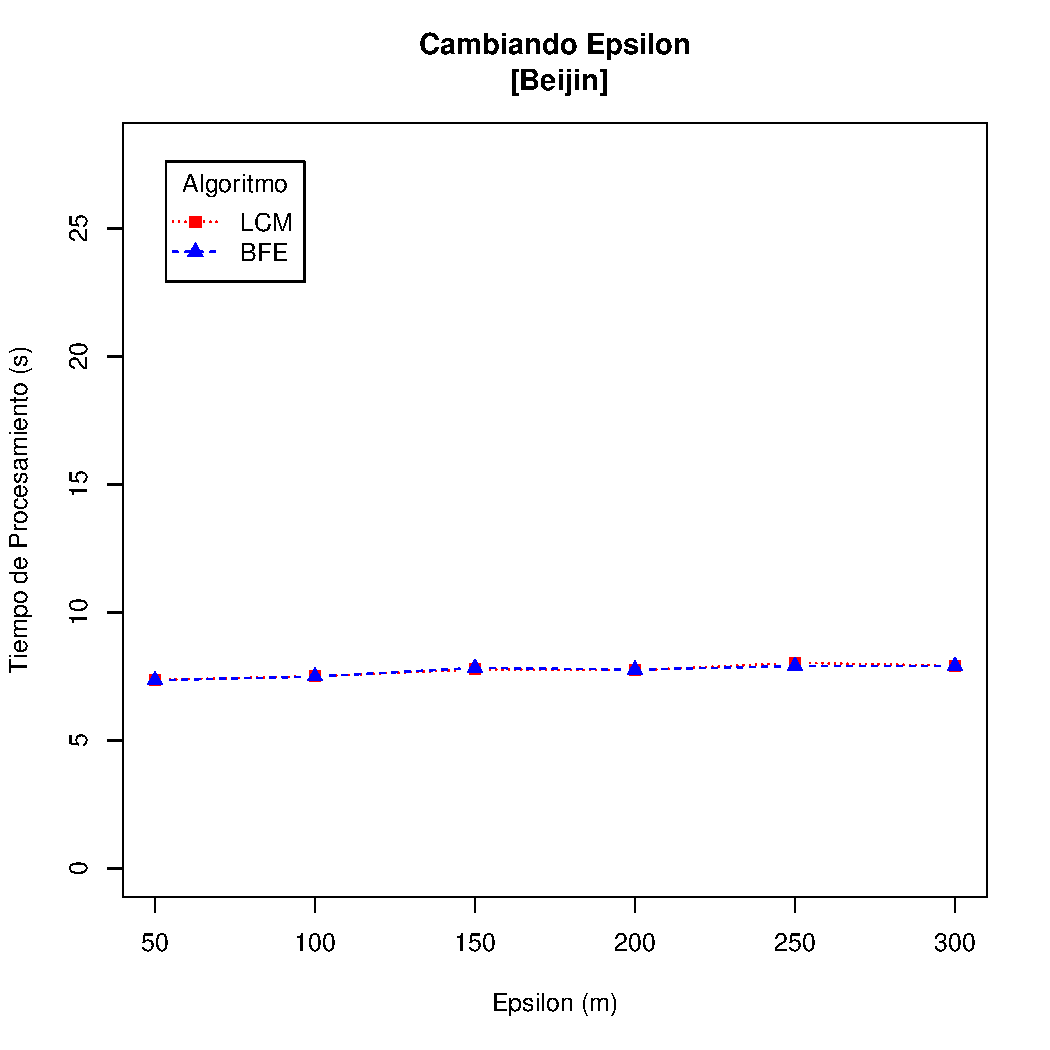
\includegraphics[scale=0.4]{pictures/Beijin.pdf}
  \caption{Caso de Prueba: Beijin}
  \label{fig:Beijin}
\end{figure}
